\subsection{Verified Example: Doubly-Linked List} \label{sec:dlist}
Rust's ownership model typically forces data structures to be acyclic,
unless they use unsafe code.
Here, we illustrate how \verb`PPtr` can be used to verify data structures that have cyclic 
pointer arrangements by verifying a double-ended queue implemented with a doubly-linked list.
Specifically, we use a doubly-linked list to represent a sequence $v_0, v_1, \ldots, v_{n-1}$,
and we implement the four operations
$\{\text{\texttt{push}}, \text{\texttt{pop}}\}
\times
\{\text{\texttt{front}}, \text{\texttt{back}}\}$.
The $i$th node in the list has both a \verb`prev` and \verb`next` pointer alongside
a single element of the sequence, $v_i$. The top level datatype, \verb`DList`, contains
\verb`head` and \verb`tail` pointers, pointing to the first and last nodes, respectively.
The full version (which can be found in our supplementary materials~\cite{verussupplementary})
contains an additional space-saving optimization,
where each node does not store its two pointers separately, but rather, stores their bitwise XOR.

\begin{figure}
    \begin{subfigure}{.48\textwidth}
      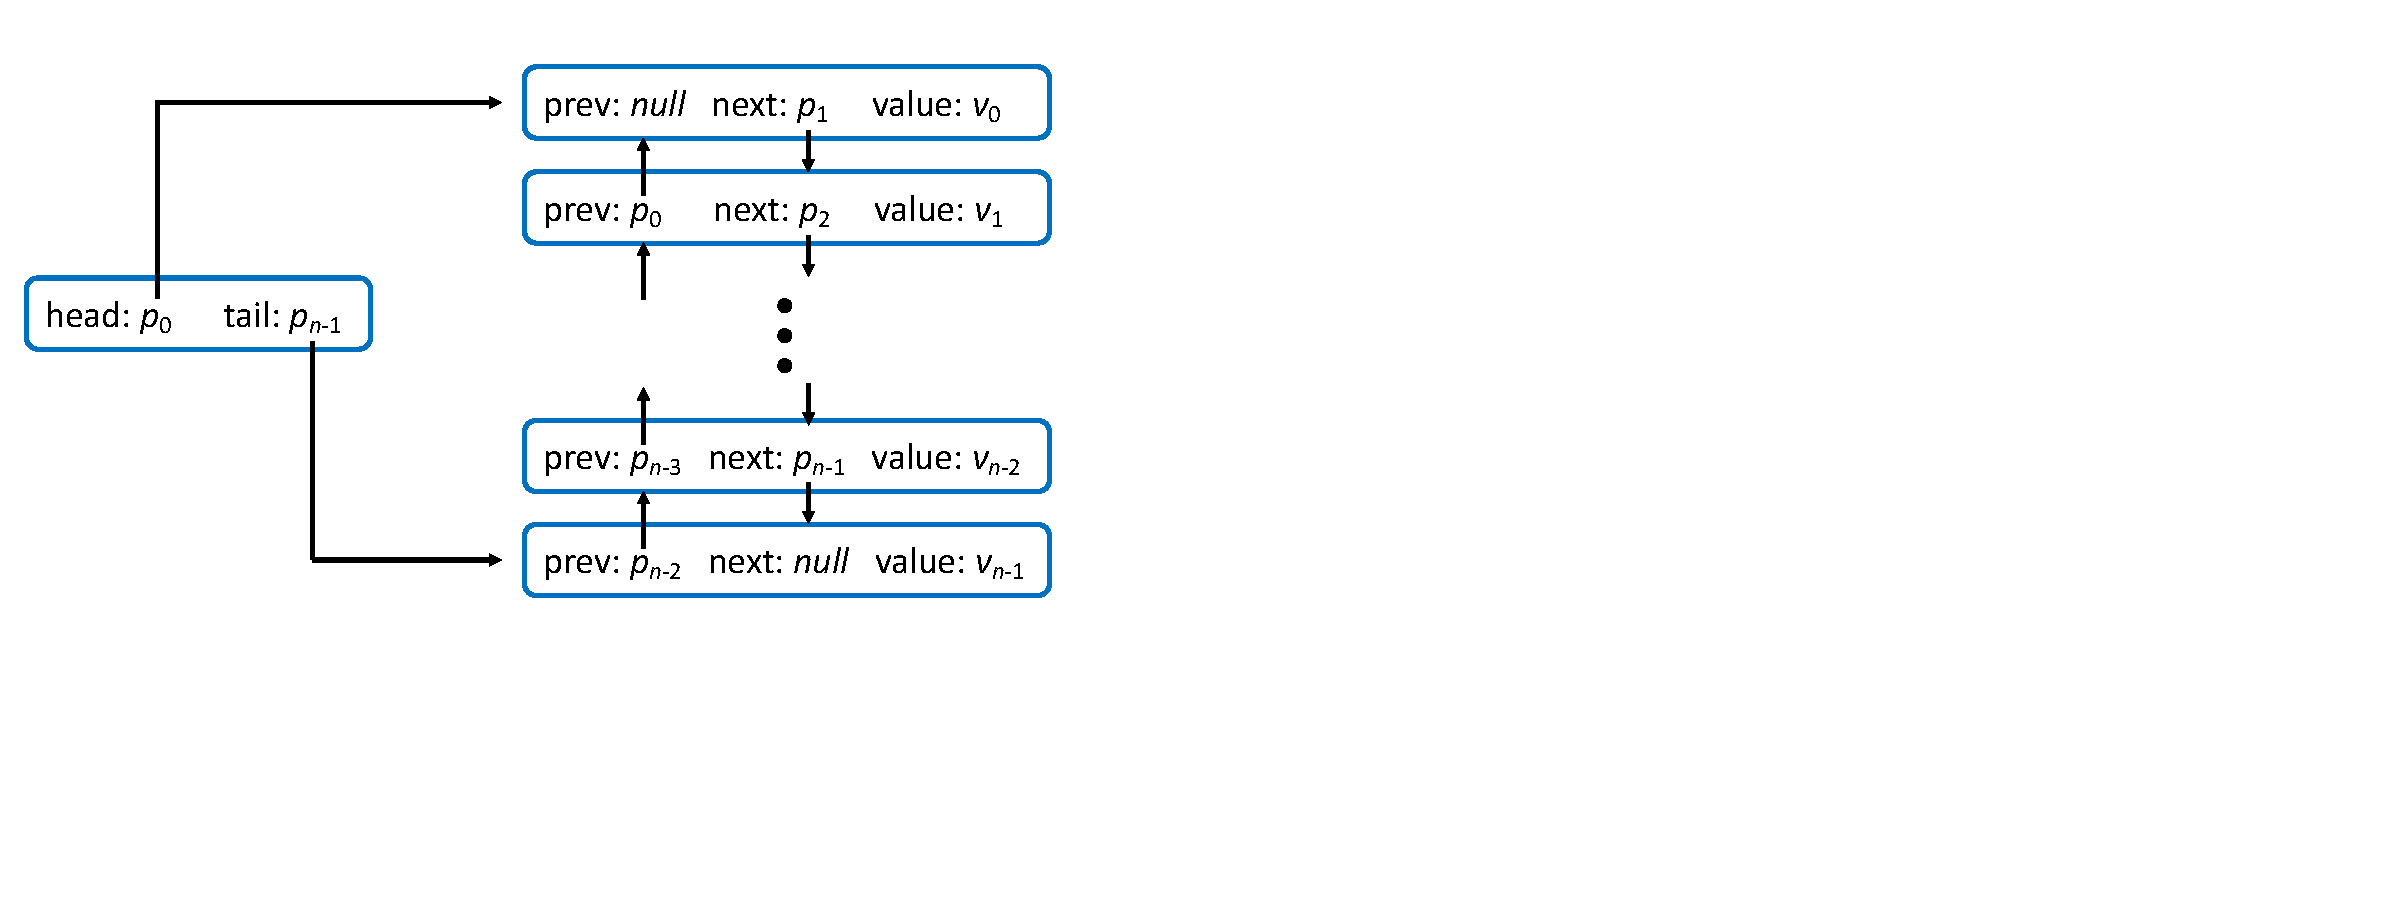
\includegraphics[width=\textwidth]{dlist-diagram-left.pdf}
      \caption{Physical pointer structure of a doubly-linked list.} \label{fig:dlist:phys}
    \end{subfigure}
    \hfill
    \begin{subfigure}{.48\textwidth}
      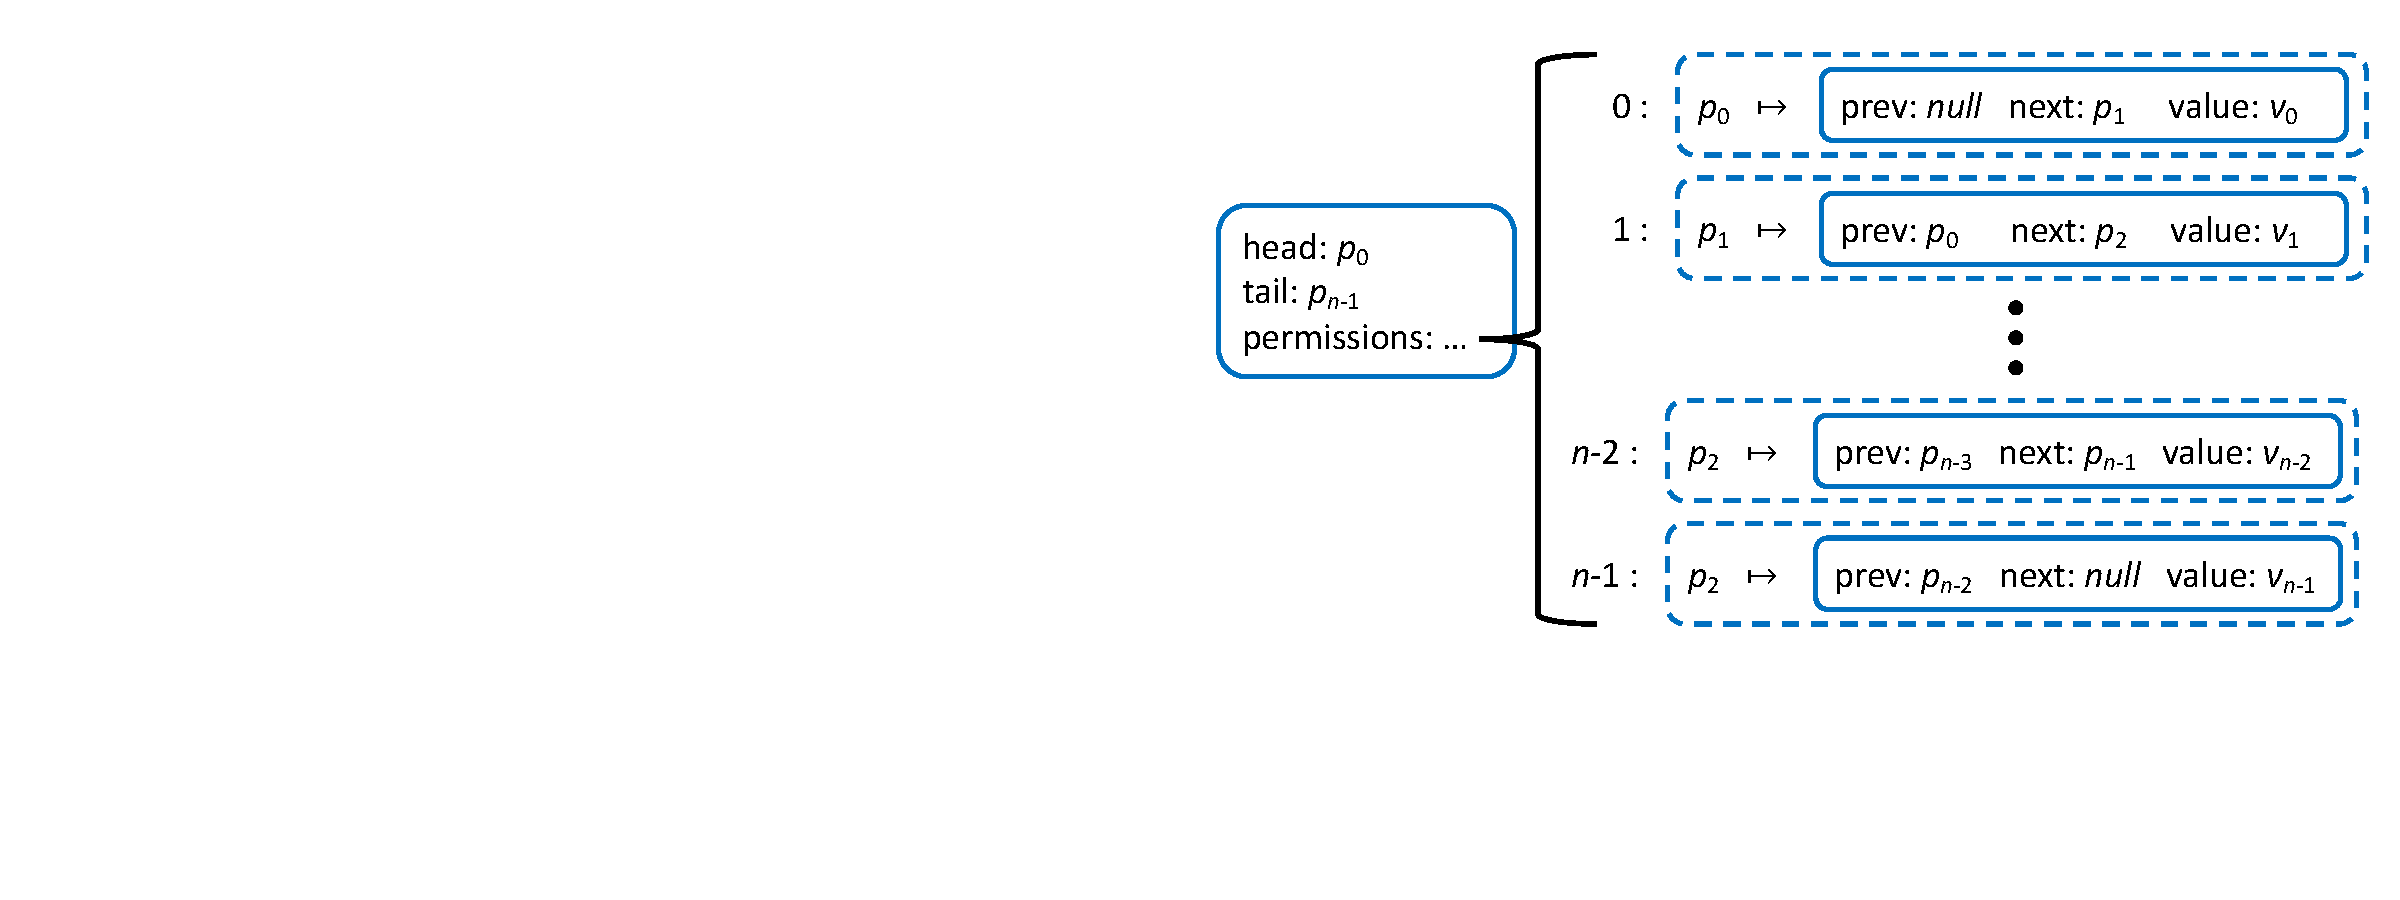
\includegraphics[width=\textwidth]{dlist-diagram-right.pdf}
      \caption{Ownership structure of a \verus doubly-linked list, which includes ghost state.} \label{fig:dlist:ghost}

    \end{subfigure}
    \caption{Doubly-linked lists. The dashed boxes are ghost, \texttt{proof}-mode \texttt{PermData} objects.} \label{fig:dlist}
\end{figure}

\begin{figure}

\begin{subfigure}{.48\textwidth}
\begin{lstlisting}[language=Verus,style=VerusLineNos]
struct Node<V> {
    prev: Option<PPtr<Node<V>>>,
    next: Option<PPtr<Node<V>>>,
    value: V,
}

struct DList<V> {
    #[spec] ptrs: Seq<PPtr<Node<V>>>,
    #[proof] perms: Map<nat, PermData<Node<V>>>,
    #[exec] head: Option<PPtr<Node<V>>>,
    #[exec] tail: Option<PPtr<Node<V>>>,
}

impl<V> DList<V> {
    #[spec] fn view(&self) -> Seq<V> { /* ... */ }

    #[exec] fn new() -> Self {
        ensures(|s: Self| s.well_formed(),
            && s.view().len() == 0); %*\lclnum\label{clnum:dlist:new}*
        /* ... */
    }

    #[exec] fn push_back(&mut self, v: V) {
        requires(old(self).well_formed());
        ensures(self.well_formed() && %*\lclnum\label{clnum:dlist:push-back}*
            equal(self.view(), old(self).view().push(v)));
        /* ... */
    }

    /* push_front, pop_back, pop_front similar */
}

fn main() {
    let mut t = DList::<u32>::new();
    t.push_back(2);   // 2
    t.push_back(3);   // 2, 3
    t.push_front(1);  // 1, 2, 3
    let x = t.pop_back();  // returns 3
    let y = t.pop_front(); // returns 1
    let z = t.pop_front(); // returns 2
    assert(x == 3);
    assert(y == 1);
    assert(z == 2);
}
\end{lstlisting}
\caption{Definition of the \texttt{DList} struct for the doubly-linked list example,
        along with the double-ended queue API, and example usage.} \label{fig:dlist:code:defn}
\end{subfigure}\hfill
\begin{subfigure}{.48\textwidth}
\begin{lstlisting}[language=Verus,style=VerusLineNos]
impl<V> DList<V> {
    #[spec] fn prev_of(&self, i: nat)
            -> Option<PPtr<Node<V>>> {
        if i == 0 {
            None
        } else {
            Some(self.ptrs.index(i as int - 1))
        }
    }

    #[spec] fn next_of(&self, i: nat)
            -> Option<PPtr<Node<V>>> {
        if i + 1 == self.ptrs.len() {
            None
        } else {
            Some(self.ptrs.index(i as int + 1))
        }
    }

    #[spec] fn wf_perm(&self, i: nat) -> bool { %*\lclnum\label{clnum:dlist:wf-perm}*
        self.perms.dom().contains(i) %*\lclnum\label{clnum:dlist:wf-perm-dom}*
        && equal(self.perms.index(i).view().pptr,
            self.ptrs.index(i as int).id()) %*\lclnum\label{clnum:dlist:wf-perm-id}*
        && match self.perms.index(i).view().value {
            Some(node) => %*\lclnum\label{clnum:dlist:wf-perm-prev-next}*
                equal(node.prev, self.prev_of(i)) &&
                equal(node.next, self.next_of(i)),
            None => false,
        }
    }

    #[spec] fn well_formed(&self) -> bool { %*\lclnum\label{clnum:dlist:well-formed}*
        (if self.ptrs.len() != 0 {
            equal(self.head, Some(self.ptrs.index(0))) && %*\lclnum\label{clnum:dlist:well-formed-head-tail}*
            equal(self.tail, Some(self.ptrs.index(self.ptrs.len() as int - 1)))
        } else {
            equal(self.head, None) && %*\lclnum\label{clnum:dlist:well-formed-head-tail-none}*
            equal(self.tail, None)
        })
        && forall(|i: nat| imply(0 <= i && i < self.ptrs.len(), self.wf_perm(i))) %*\lclnum\label{clnum:dlist:well-formed-forall}*
    }
}
\end{lstlisting}
\caption{Definition of \texttt{well\_formed}, used internally by the \texttt{DList}
         implementation to prove correctness of \texttt{push\_back} and others.} \label{fig:dlist:code:wf}
\end{subfigure}
    \caption{Doubly-linked list example} \label{fig:dlist:code}
\end{figure}

\autoref{fig:dlist:phys} shows the physical pointer structure of the list.
However, the diagram does not properly reflect a valid ownership structure
because it shows each node with multiple incoming pointers.
%
In the \verus implementation, we include an additional field in \verb`DList`:
the ghost \verb`permissions` field, which maintains permissions for \emph{every} node
in the doubly-linked list via a simple ``flattened'' structure, as in \autoref{fig:dlist:ghost}.
Specifically, for each $i \in \{0,\ldots,n-1\}$, we maintain a \verb`PermData` object
that maps pointer $p_i$ to the value it points to: the content of $i$th node, which contains
$v_i$ and the appropriate pointers, \verb`prev` as $p_{i-1}$ and \verb`next` as $p_{i+1}$.
To traverse the doubly-linked list, a user may use \verb`head` to determine $p_0$,
dereference $p_0$ using the $0$th permission object, find $p_1$, and so on.
In other words, we ghostily track the entire state of the list, but to get the same data in \emph{exec-mode}, we need to actually walk the pointers.

\autoref{fig:dlist:code} shows a snippet of the API. The spec-mode \verb`view()` function provides an abstraction
of the list as a simple sequence $v_0, v_1, \ldots, v_{n-1}$.
The specifications of the exec-mode API functions are all given in terms of this abstraction.
For example, the postcondition of \verb`DList::new()` says that the list represents the empty sequence,
while the postcondition of \verb`DList::push_front(v)` says that \verb`v` is appended to the end of the sequence.
The remaining three API functions (\verb`push_back`, \verb`pop_front`, and \verb`pop_back`) are similar.

The exec implementations are too involved to show here, so instead we show the definition of
the spec-mode predicate \verb`well_formed`~\lclref{clnum:dlist:well-formed},
i.e., the invariant that holds on \verb`DList<T>` and which each operation must preserve.
This definition says that~\lclref{clnum:dlist:well-formed-head-tail} the \verb`head` and \verb`tail` pointers are the first and last, respectively
(unless the list is empty, in which case~\lclref{clnum:dlist:well-formed-head-tail-none} they are both \verb`None`).
Finally, the \verb`forall`~\lclref{clnum:dlist:well-formed-forall} says that for each $0 \le i < n$, \verb`wf_perm(i)` holds; i.e.,
the $i$th permission is correct.
The definition of \verb`wf_perm(i)`~\lclref{clnum:dlist:wf-perm} says that
the permission is in our \verb`perms` map~\lclref{clnum:dlist:wf-perm-dom},
the permission corresponds to $p_i$~\lclref{clnum:dlist:wf-perm-id},
and that the \verb`prev` and \verb`next` fields of the node have the correct values~\lclref{clnum:dlist:wf-perm-prev-next}.


